\documentclass[12pt,letterpaper]{article}
\usepackage{graphicx,textcomp}
\usepackage{natbib}
\usepackage{setspace}
\usepackage{fullpage}
\usepackage{color}
\usepackage[reqno]{amsmath}
\usepackage{amsthm}
\usepackage{fancyvrb}
\usepackage{amssymb,enumerate}
\usepackage[all]{xy}
\usepackage{endnotes}
\usepackage{lscape}
\newtheorem{com}{Comment}
\usepackage{float}
\usepackage{hyperref}
\newtheorem{lem} {Lemma}
\newtheorem{prop}{Proposition}
\newtheorem{thm}{Theorem}
\newtheorem{defn}{Definition}
\newtheorem{cor}{Corollary}
\newtheorem{obs}{Observation}
\usepackage[compact]{titlesec}
\usepackage{dcolumn}
\usepackage{tikz}
\usetikzlibrary{arrows}
\usepackage{multirow}
\usepackage{subcaption}
\usepackage{xcolor}
\newcolumntype{.}{D{.}{.}{-1}}
\newcolumntype{d}[1]{D{.}{.}{#1}}
\definecolor{light-gray}{gray}{0.65}
\usepackage{url}
\usepackage{listings}
\usepackage{color}
\definecolor{codegreen}{rgb}{0,0.6,0}
\definecolor{codegray}{rgb}{0.5,0.5,0.5}
\definecolor{codepurple}{rgb}{0.58,0,0.82}
\definecolor{backcolour}{rgb}{0.95,0.95,0.92}

\lstdefinestyle{mystyle}{
	backgroundcolor=\color{backcolour},   
	commentstyle=\color{codegreen},
	keywordstyle=\color{magenta},
	numberstyle=\tiny\color{codegray},
	stringstyle=\color{codepurple},
	basicstyle=\footnotesize,
	breakatwhitespace=false,         
	breaklines=true,                 
	captionpos=b,                    
	keepspaces=true,                 
	numbers=left,                    
	numbersep=5pt,                  
	showspaces=false,                
	showstringspaces=false,
	showtabs=false,                  
	tabsize=2
}
\lstset{style=mystyle}
\newcommand{\Sref}[1]{Section~\ref{#1}}

\title{ Price House Group Project}
\date{November 16th, 2022}
\author{Group A}

\begin{document}
	\maketitle
	
\section{Data Transformation}

\lstinputlisting[language=R, firstline=148, lastline=150]{Week 9 R train.R}  


% Table created by stargazer v.5.2.3 by Marek Hlavac, Social Policy Institute. E-mail: marek.hlavac at gmail.com% Date and time: Wed, Nov 16, 2022 - 13:55:14

\begin{table}[!htbp] \centering   \caption{}   \label{} 
	\begin{tabular}{@{\extracolsep{5pt}}lc} \\[-1.8ex]\hline \hline \\[-1.8ex]  & \multicolumn{1}{c}{\textit{Dependent variable:}} \\ \cline{2-2} \\[-1.8ex] & SqFtLot \\ \hline \\[-1.8ex]  SqFtTotLiving & 5.898$^{***}$ \\   & (0.220) \\   & \\  ZipGroup & $-$47.632$^{***}$ \\   & (3.848) \\   & \\  Constant & 4,671,229.000$^{***}$ \\   & (377,536.400) \\   & \\ \hline \\[-1.8ex] Observations & 20,340 \\ R$^{2}$ & 0.049 \\ Adjusted R$^{2}$ & 0.049 \\ Residual Std. Error & 28,158.290 (df = 20337) \\ F Statistic & 522.163$^{***}$ (df = 2; 20337) \\ \hline \hline \\[-1.8ex] \textit{Note:}  & \multicolumn{1}{r}{$^{*}$p$<$0.1; $^{**}$p$<$0.05; $^{***}$p$<$0.01} \\ 
\end{tabular} 
\end{table} 

 \vspace{.25cm}

% Table created by stargazer v.5.2.3 by Marek Hlavac, Social Policy Institute. E-mail: marek.hlavac at gmail.com% Date and time: Wed, Nov 16, 2022 - 14:12:09
\begin{table}[!htbp] \centering   \caption{}   \label{} \begin{tabular}{@{\extracolsep{5pt}}lc} \\[-1.8ex]\hline \hline \\[-1.8ex]  & \multicolumn{1}{c}{\textit{Dependent variable:}} \\ \cline{2-2} \\[-1.8ex] & AdjSalePrice \\ \hline \\[-1.8ex]  SqFtTotLiving & 186.719$^{***}$ \\   & (3.169) \\   & \\  BldgGrade & 115,699.300$^{***}$ \\   & (2,453.317) \\   & \\  ZipGroup & 647.235$^{***}$ \\   & (36.013) \\   & \\  Constant & $-$64,191,980.000$^{***}$ \\   & (3,533,963.000) \\   & \\ \hline \\[-1.8ex] Observations & 20,340 \\ R$^{2}$ & 0.539 \\ Adjusted R$^{2}$ & 0.539 \\ Residual Std. Error & 262,916.700 (df = 20336) \\ F Statistic & 7,928.905$^{***}$ (df = 3; 20336) \\ \hline \hline \\[-1.8ex] \textit{Note:}  & \multicolumn{1}{r}{$^{*}$p$<$0.1; $^{**}$p$<$0.05; $^{***}$p$<$0.01} \\ 
\end{tabular} 
\end{table} 

% Table created by stargazer v.5.2.3 by Marek Hlavac, Social Policy Institute. E-mail: marek.hlavac at gmail.com% Date and time: Wed, Nov 16, 2022 - 14:34:18
\begin{table}[!htbp] \centering   \caption{}   \label{} 
	\begin{tabular}{@{\extracolsep{5pt}}lc} \\[-1.8ex]\hline \hline \\[-1.8ex]  & \multicolumn{1}{c}{\textit{Dependent variable:}} \\ \cline{2-2} \\[-1.8ex] & AdjSalePrice \\ \hline \\[-1.8ex]  SqFtTotLiving & 176.735$^{***}$ \\   & (3.012) \\   & \\  BldgGrade & 151,549.500$^{***}$ \\   & (2,460.825) \\   & \\  YrBuilt & $-$3,173.910$^{***}$ \\   & (64.355) \\   & \\  Constant & 5,289,625.000$^{***}$ \\   & (121,827.000) \\   & \\ \hline \\[-1.8ex] Observations & 20,340 \\ R$^{2}$ & 0.582 \\ Adjusted R$^{2}$ & 0.582 \\ Residual Std. Error & 250,442.000 (df = 20336) \\ F Statistic & 9,430.591$^{***}$ (df = 3; 20336) \\ \hline \hline \\[-1.8ex] \textit{Note:}  & \multicolumn{1}{r}{$^{*}$p$<$0.1; $^{**}$p$<$0.05; $^{***}$p$<$0.01} \\ 
\end{tabular} 
\end{table} 


\section{ Residual}


\noindent Residual  \\

 \vspace{.25cm}
 
 \lstinputlisting[language=R, firstline=75, lastline=77]{Week 9 R train.R}  



\section{Summary}

Data Summary on SqFtTotLiving
\begin{tabbing}
	
	   Min. 1st Qu.  Median    Mean 3rd Qu.    Max.     
	370    1420    1910    2079    2540   10740 
	
\end{tabbing}


\vspace{.25cm}

\begin{figure}
[h!]\centering
\caption{\footnotesize Plot.}
\label{fig:plot_1}
\includegraphics[width=.85\textwidth]{Rplot_pairs.pdf}
\end{figure}

\vspace{.25cm}

\begin{figure}
	[h!]\centering
	\caption{\footnotesize Plot.}
	\label{fig:plot_1}
	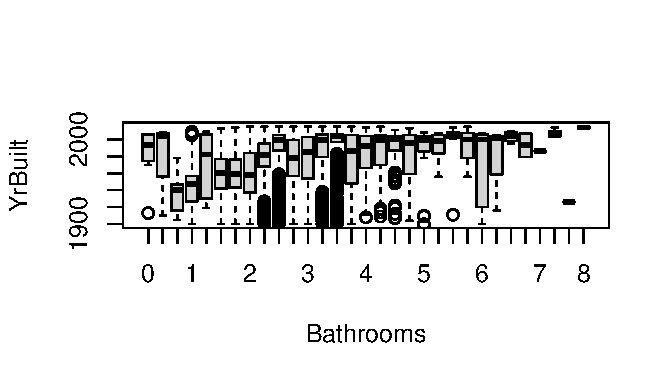
\includegraphics[width=.85\textwidth]{Rplot01.pdf}
\end{figure}



\end{document}

